%\documentclass[11pt, oneside]{article}   	
%\usepackage{geometry}    
%\geometry{letterpaper}                 		
\input preamble.tex
\newcommand{\ig}[2][width=4in]{\includegraphics[#1]{#2}}    		
\usepackage{graphicx}					
\usepackage{amssymb}
\usepackage{pgfplotstable}
\usepackage{float}
\usepackage{caption}
\captionsetup[table]{justification=justified,singlelinecheck=false, position=bottom}
\begin{document}

\header {\today}							
\title{Muon Lifetime}
\author{Ekta Patel \& Brandon Booth-Dunbar}

\section{Abstract}
%Ekta
\begin{em} Positively charged muons reach the Earth via cosmic ray showers.When they decay, the muons break down into a positron, an electron neutrino and a muon neutrino.The goal of the experiment is to measure the lifetime of the muon by detecting and stopping a positive muon in an aluminum slab and then consequently detected the positron that it leaves behind when it decays.The distribution of the difference in detection times can be used to determine the muon lifetime.
\end{em}

\section{Theory}
%Brandon

\section{Experimental Methods}
%Ekta, but I (Brandon)  will make the figures
\subsection{Apparatus}
\begin{figure}[H]
\begin{center}
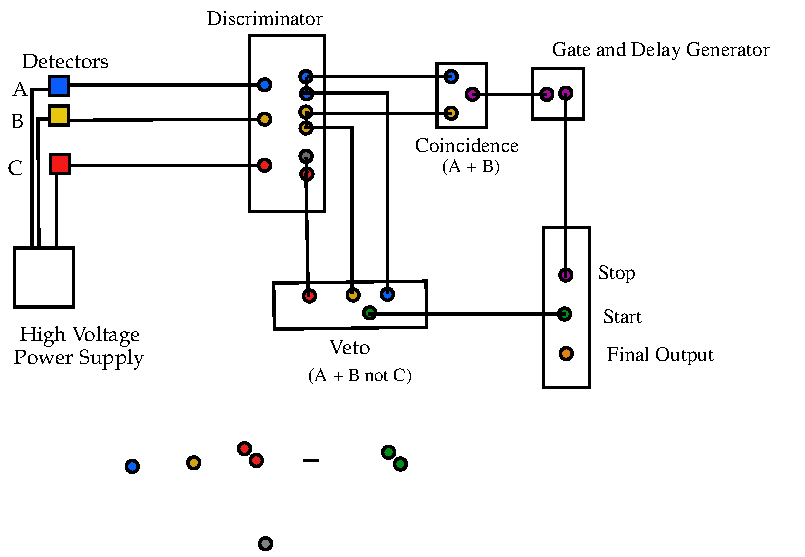
\includegraphics[width=4 in]{ML-figure1.pdf}
\caption{Bitches be figurin'}
\end{center}
\end{figure}

\subsection{Procedure}


\section{Results \& Discussion}
%Brandon

\section{Conclusion}
%Ekta

\begin{thebibliography}{99}
%\bibitem{}
\end{thebibliography}

\newpage \LARGE{Appendix}

\end{document}  
